% !TEX root = poster.tex
%\headerbox{Recent Developments}{name=devs,column=1,row=1,below=run1,above=bottom}{
\headerbox{\textbf{Developments}}{name=devs,column=1,row=1,span=2,below=run1}{
\begin{minipage}{0.474\boxwidth}
\vspace{-0.61em}
\textbf{OS charm tagger (preliminary)}\\
\vspace{-1.12em}
\begin{itemize}
\setlength\itemsep{0.01em}
\item reconstruct $D^0$/$D^\pm$/$D^*$ decays related to OS $b$ decay

\vspace{-1.4em}
\begin{center}
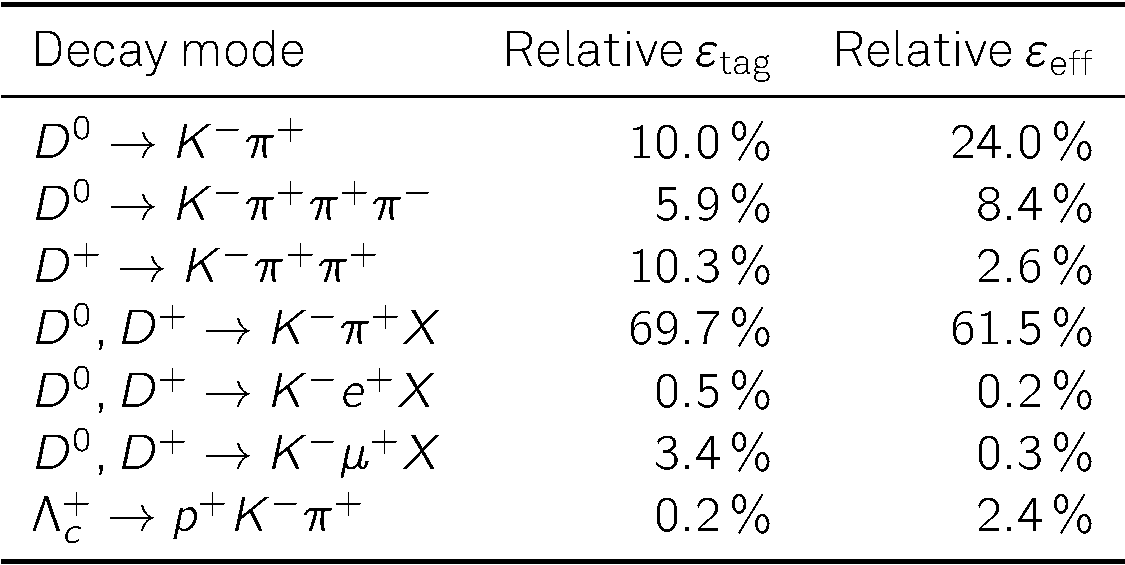
\includegraphics[width=0.802\textwidth]{figures/OSCharmTable1.pdf}
\end{center}
\vspace{-1.5em}

\item one boosted decision tree (BDT) for each mode [12]
\item clean measure of \B meson flavour (low mistag) 
\item stand-alone tagging power of $\varepsilon_{\text{eff}}=\SI{0.30}{\%}$ to \SI{0.40}{\%}
%\item analysis note in preparation
\end{itemize}

\vspace{0.3em}

\textbf{SS pion calibration}
\vspace{-0.3em}
\begin{itemize}
\setlength\itemsep{0.01em}
\item calibration performed with \BdToJPsiKst
\item full evaluation of systematic uncertainties 
\item used for the first time in the measurements of
\begin{itemize}
\setlength{\itemindent}{-.11in}
\item[${\color{tu_gruen}-}$] $\sin(2\beta)$ with $\Bd \rightarrow \jpsi K_S^0$
\setlength{\itemindent}{.05in}
%\item[${\color{tu_gruen}\Rightarrow}$] precision comparable to $B$-factories
\item[${\color{tu_gruen}\Rightarrow}$] $\varepsilon_{\text{eff}}^{\text{SS}\pion} = 0.38\,\%$
\setlength{\itemindent}{-.11in}
\item[${\color{tu_gruen}-}$] $\sin(2\beta_{\text{eff}})$ with $\Bd \rightarrow \jpsi \pi^+ \pi^-$
\setlength{\itemindent}{.05in}
\item[${\color{tu_gruen}\Rightarrow}$] $\varepsilon_{\text{eff}}^{\text{SS}\pion} = 0.54\,\%$
\end{itemize}

\end{itemize}
\vspace{-0.7em}
\end{minipage}
%\vspace{-0.1em}
\hfill
\begin{minipage}{0.474\boxwidth}
\vspace{0.25em}
\textbf{SS kaon tagging using neural nets (NN)}
\vspace{-0.42em}

\begin{itemize}
\item basic idea: use two NN
\vspace{-0.5em}
	\begin{itemize}
	\setlength\itemsep{0.01em}
	\setlength{\itemindent}{-.11in}
	\item[${\color{tu_gruen}-}$] first NN distinguishes between:
	\vspace{-0.25em}
		\begin{enumerate}
		\item fragmentation tracks\\
		${\color{tu_gruen}\Rightarrow}$ signal for SS kaon nnet
		%\item OS $b$ hadron tracks\\
		%${\color{tu_gruen}\Rightarrow}$ signal for OS kaon nnet
		\item underlying event tracks 
		\end{enumerate}
	\end{itemize}
\vspace{-1.7em}

\begin{flushleft}
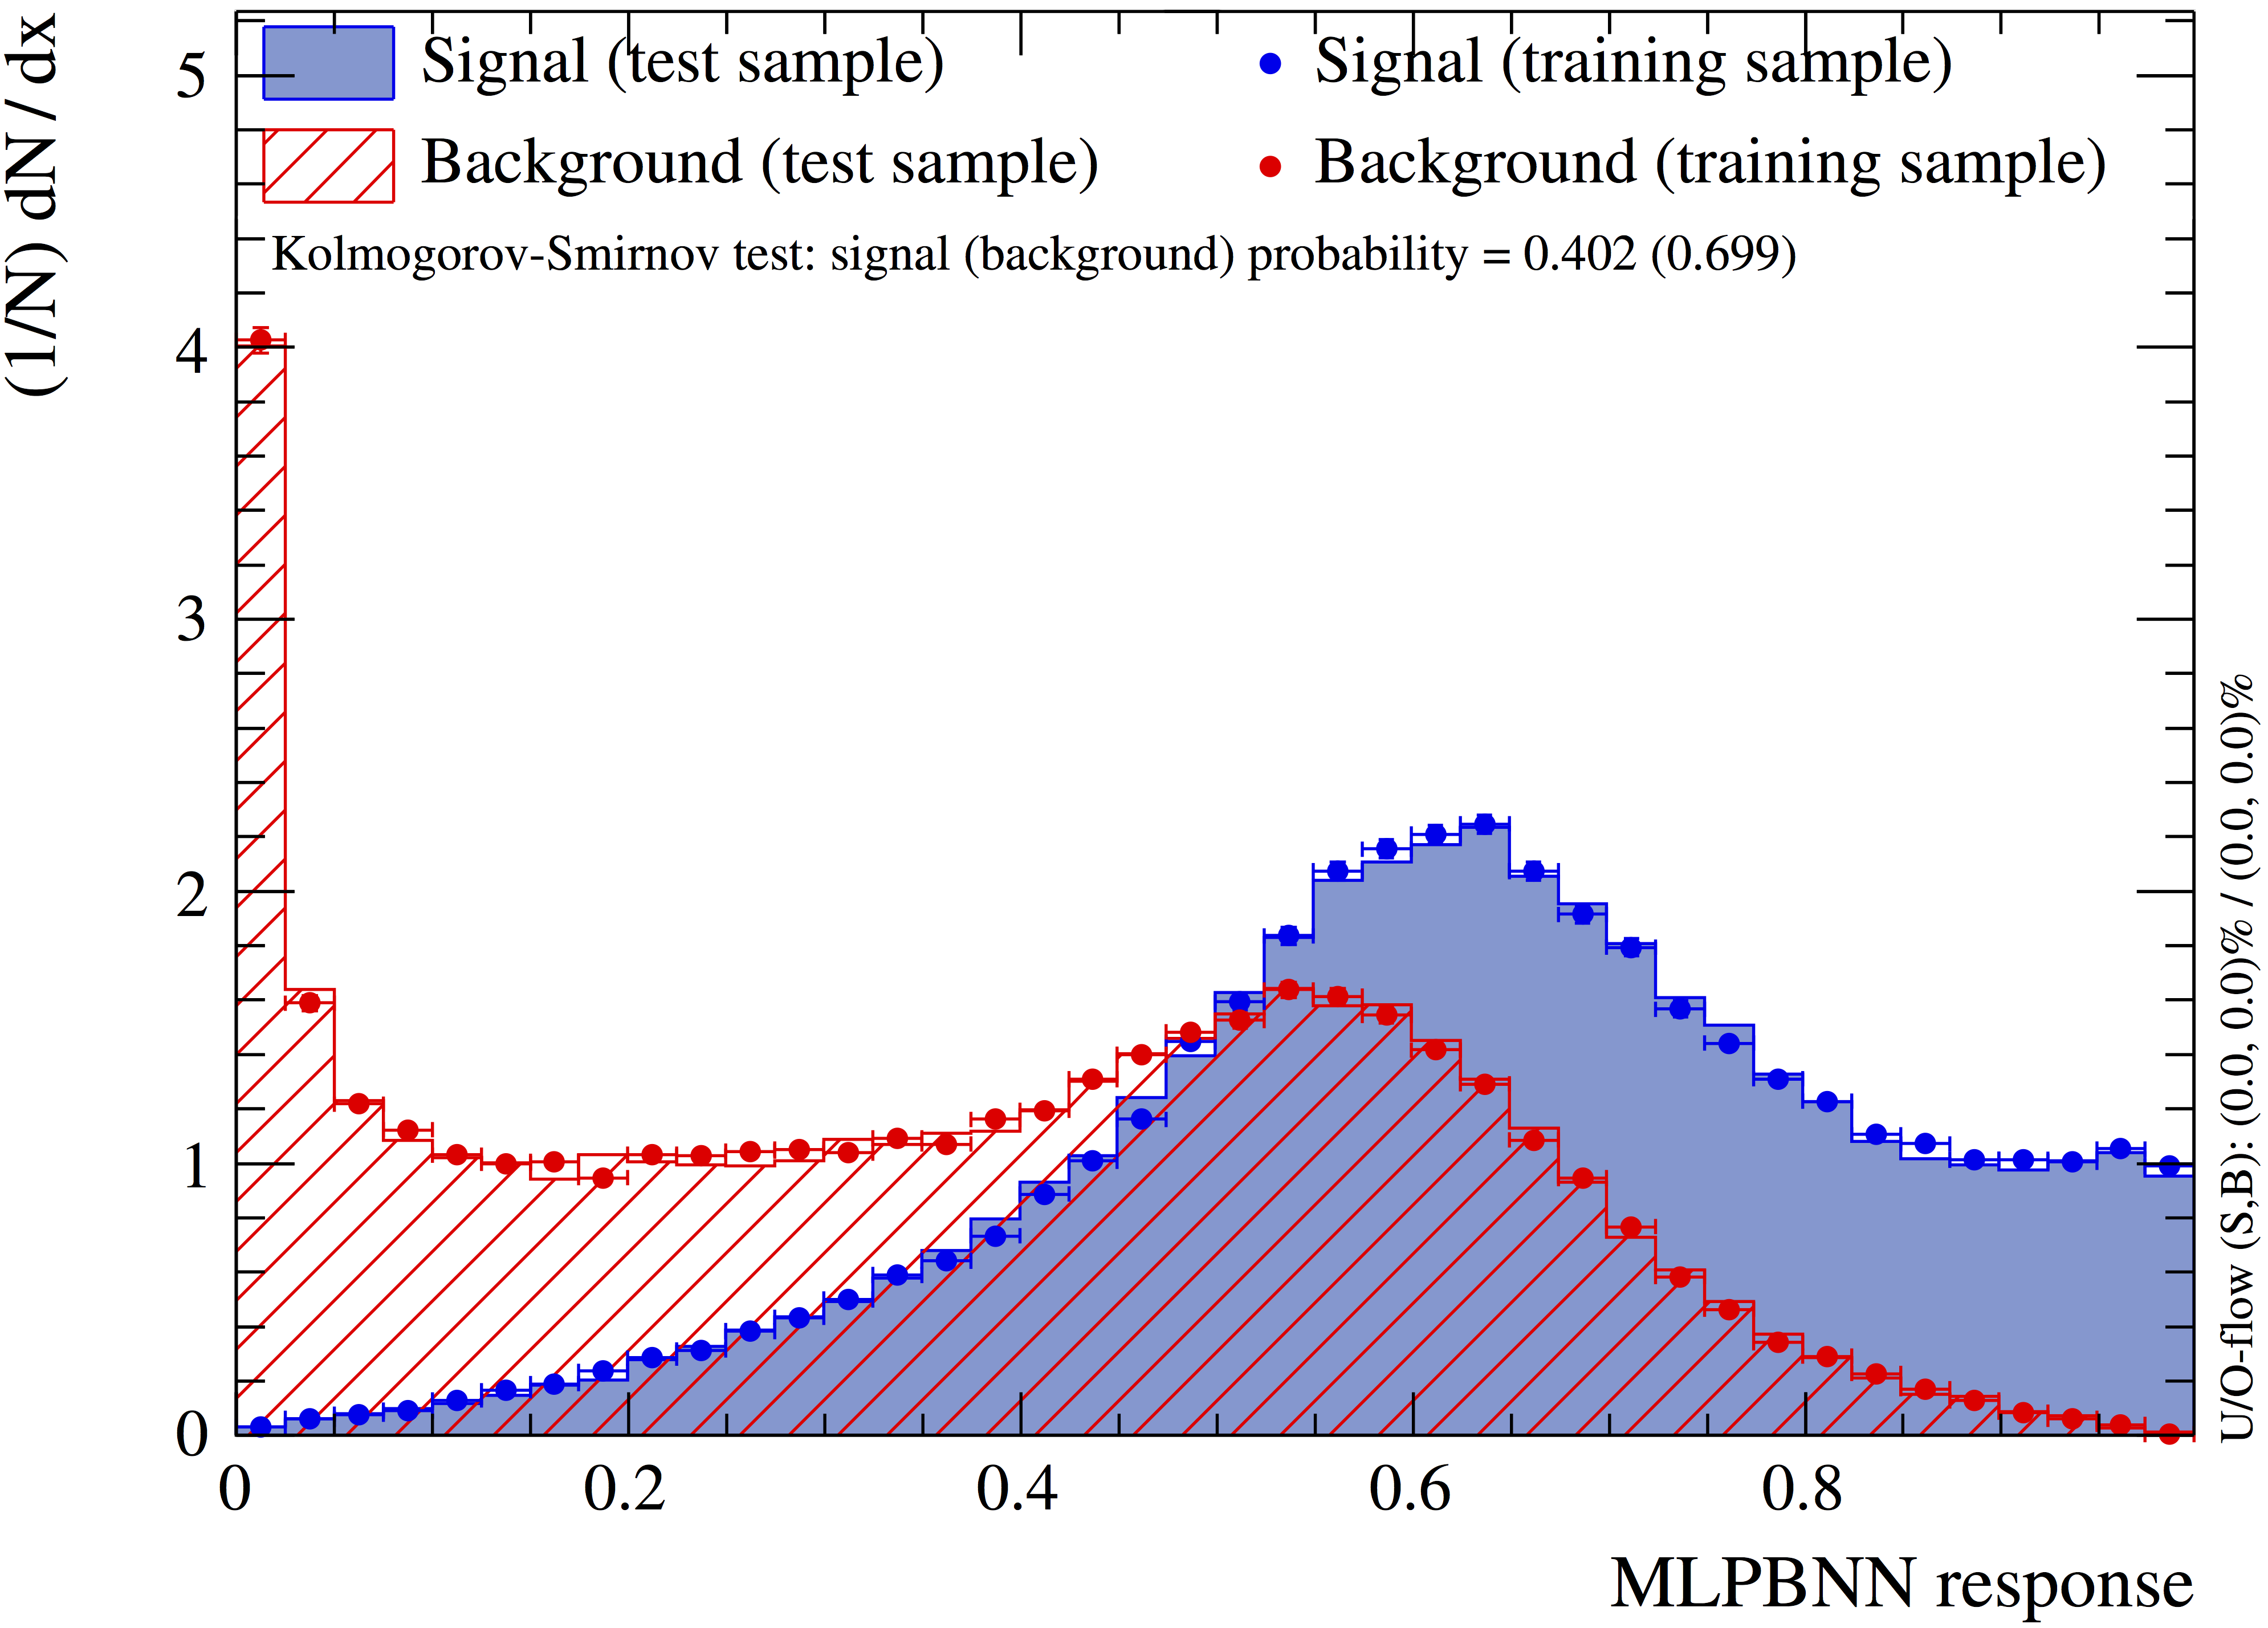
\includegraphics[width=0.802\textwidth]{figures/sskaonNnetfirstNN3.png}
\end{flushleft}

\vspace{-2.3em}

\setlength\itemsep{0.01em}
\setlength{\itemindent}{-.11in}
\begin{itemize}
\setlength{\itemindent}{-.11in}
\item[${\color{tu_gruen}-}$] second NN:
\begin{itemize}
%\item[${\color{tu_gruen}\circ}$] receives up to 3 candidates 
\item[${\color{tu_gruen}\circ}$] assigns final tag and mistag  based\\ on multiple candidates [13]
\end{itemize}
\end{itemize}
\end{itemize}
\vspace{-1.75em}
\begin{itemize}
\setlength\itemsep{0.01em}
%\item both taggers have a high efficiency
\item SS kaon nnet tagger is a great success, compared \newline to the previous cut-based SS kaon it gives  
\begin{itemize}
\setlength{\itemindent}{-.11in}
\vspace{-0.5em}
\item[${\color{tu_gruen}-}$] \BsToDspi: $50\,\%$ relative improvement in $\varepsilon_{\text{eff}}$
\item[${\color{tu_gruen}-}$] \BsToJPsiPhi: $41\,\%$ relative improvement in $\varepsilon_{\text{eff}}$
\end{itemize}
\end{itemize}
%\vspace{-0.1em}
\vspace{-0.75em}
\end{minipage}
}




%combine NNet Tagger chapters